\documentclass[12pt, a4paper]{article}

% ── Packages ──────────────────────────────────────────────────────
\usepackage[utf8]{inputenc}
\usepackage[T1]{fontenc}
\usepackage{amsmath, amssymb, amsthm}
\usepackage{mathtools}
\usepackage{enumitem}
\usepackage{tikz}
\usetikzlibrary{calc, positioning, arrows.meta, fit, patterns, decorations.pathreplacing}
\usepackage{geometry}
\geometry{margin=2.4cm}
\usepackage{xcolor}
\usepackage{tcolorbox}
\tcbuselibrary{theorems, skins, breakable}
\usepackage{booktabs}
\usepackage{hyperref}
\hypersetup{colorlinks=true, linkcolor=blue!60!black, urlcolor=blue!60!black}

\setlength{\parindent}{0pt}
\setlength{\parskip}{6pt}

% ── Colours ───────────────────────────────────────────────────────
\definecolor{setA}{RGB}{66, 133, 244}   % blue
\definecolor{setB}{RGB}{234, 67, 53}    % red
\definecolor{setC}{RGB}{251, 188, 4}    % yellow
\definecolor{theoryBg}{RGB}{232, 245, 253}
\definecolor{theoryFrame}{RGB}{66, 133, 244}
\definecolor{stmtBg}{RGB}{255, 243, 224}
\definecolor{stmtFrame}{RGB}{230, 126, 34}
\definecolor{ansBg}{RGB}{232, 250, 232}
\definecolor{ansFrame}{RGB}{39, 174, 96}

% ── Environments ──────────────────────────────────────────────────
\newtcolorbox{theorybox}[1][]{%
  colback=theoryBg, colframe=theoryFrame,
  fonttitle=\bfseries, title={\small Theory Recap: #1},
  breakable, enhanced, arc=2mm,
  left=5pt, right=5pt, top=5pt, bottom=5pt
}

\newtcolorbox{problembox}{%
  colback=stmtBg, colframe=stmtFrame,
  fonttitle=\bfseries, title={\small Problem Statement},
  breakable, enhanced, arc=2mm,
  left=5pt, right=5pt, top=5pt, bottom=5pt
}

\newtcolorbox{answerbox}{%
  colback=ansBg, colframe=ansFrame,
  arc=2mm, left=5pt, right=5pt, top=3pt, bottom=3pt
}

\newcommand{\Z}{\mathbb{Z}}
\newcommand{\R}{\mathbb{R}}
\newcommand{\N}{\mathbb{N}}
\newcommand{\powset}[1]{2^{#1}}
\newcommand{\comp}[1]{\overline{#1}}
\newcommand{\symdiff}{\mathbin{\triangle}}

% ── Title ─────────────────────────────────────────────────────────
\title{\textbf{Practice 1 --- Set Theory}\\[4pt]
       \large Solutions to Selected Problems\\[2pt]
       \normalsize Problems 2, 7, 11, 16, 20, 54\,(3,\,11), 58, 60}
\author{Discrete Mathematics --- QYSU}
\date{}

\begin{document}
\maketitle
\tableofcontents
\newpage

% ══════════════════════════════════════════════════════════════════
\section{Problem 2 --- Membership with $\emptyset$ and $\{\emptyset\}$}
% ══════════════════════════════════════════════════════════════════

\begin{theorybox}[Membership ($\in$) vs.\ Subset ($\subseteq$)]
These two relations are fundamentally different:
\begin{itemize}[nosep]
  \item $a \in S$ means ``$a$ is an \textbf{element} of $S$.''
  \item $A \subseteq S$ means ``every element of $A$ is also in $S$.''
\end{itemize}

\medskip
The empty set $\emptyset$ has no elements.
The set $\{\emptyset\}$ is \textbf{not} empty---it has one element, namely $\emptyset$ itself.
To decide ``$x \in S$\,?'' list the elements of $S$ and check whether $x$ is one of them.

\begin{center}
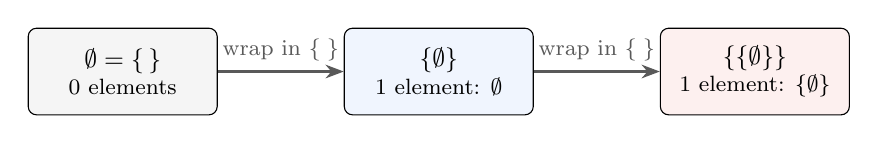
\begin{tikzpicture}[
  box/.style={draw, rounded corners=3pt, minimum width=2.4cm,
              minimum height=1.1cm, align=center, font=\small},
  >=Stealth
]
  \node[box, fill=gray!8] (e0)
    {$\emptyset = \{\,\}$\\[-1pt]\footnotesize 0 elements};
  \node[box, fill=setA!8, right=1.6cm of e0] (e1)
    {$\{\emptyset\}$\\[-1pt]\footnotesize 1 element: $\emptyset$};
  \node[box, fill=setB!8, right=1.6cm of e1] (e2)
    {$\{\{\emptyset\}\}$\\[-1pt]\footnotesize 1 element: $\{\emptyset\}$};
  \draw[->, thick, gray!70!black] (e0) -- (e1)
    node[midway, above, font=\footnotesize]{wrap in $\{\;\}$};
  \draw[->, thick, gray!70!black] (e1) -- (e2)
    node[midway, above, font=\footnotesize]{wrap in $\{\;\}$};
\end{tikzpicture}
\end{center}
Each wrapping step creates a new set whose sole element is the previous set.
\end{theorybox}

\begin{problembox}
Which of the following statements are true?
\begin{enumerate}[label=2.\arabic*.]
  \item $\emptyset \in \{\emptyset,\; \{\emptyset\}\}$
  \item $\{\emptyset\} \in \{\{\emptyset\}\}$
  \item $\emptyset \in \{\{\emptyset\}\}$
\end{enumerate}
\end{problembox}

\subsection*{Solution}

The strategy is always the same: \emph{list the elements} of the outer set,
then check whether the object on the left of $\in$ matches any of them.

\begin{center}
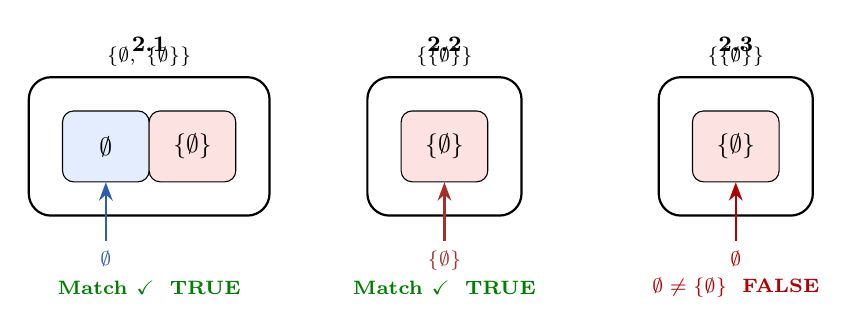
\begin{tikzpicture}[
  elem/.style={draw, rounded corners=4pt, minimum width=1.1cm,
               minimum height=0.9cm, inner sep=2pt, font=\small, align=center},
  container/.style={draw, rounded corners=8pt, inner sep=12pt, thick},
  >=Stealth
]
  % ── 2.1 ──
  \begin{scope}[xshift=0cm]
    \node[font=\footnotesize\bfseries] at (0.55, 2.0) {2.1};
    \node[elem, fill=setA!15] (a1) at (0, 0.7) {$\emptyset$};
    \node[elem, fill=setB!15] (a2) at (1.1, 0.7) {$\{\emptyset\}$};
    \node[container, fit=(a1)(a2),
          label={[font=\scriptsize]above:$\{\emptyset,\;\{\emptyset\}\}$}] {};
    \draw[->, thick, setA!70!black]
      (0, -0.5) node[below, font=\scriptsize]{$\emptyset$} -- (a1.south);
    \node[font=\scriptsize\bfseries, green!50!black] at (0.55, -1.1)
      {Match $\checkmark$ \;\textbf{TRUE}};
  \end{scope}

  % ── 2.2 ──
  \begin{scope}[xshift=4.3cm]
    \node[font=\footnotesize\bfseries] at (0, 2.0) {2.2};
    \node[elem, fill=setB!15] (b1) at (0, 0.7) {$\{\emptyset\}$};
    \node[container, fit=(b1),
          label={[font=\scriptsize]above:$\{\{\emptyset\}\}$}] {};
    \draw[->, thick, setB!70!black]
      (0, -0.5) node[below, font=\scriptsize]{$\{\emptyset\}$} -- (b1.south);
    \node[font=\scriptsize\bfseries, green!50!black] at (0, -1.1)
      {Match $\checkmark$ \;\textbf{TRUE}};
  \end{scope}

  % ── 2.3 ──
  \begin{scope}[xshift=8cm]
    \node[font=\footnotesize\bfseries] at (0, 2.0) {2.3};
    \node[elem, fill=setB!15] (c1) at (0, 0.7) {$\{\emptyset\}$};
    \node[container, fit=(c1),
          label={[font=\scriptsize]above:$\{\{\emptyset\}\}$}] {};
    \draw[->, thick, red!70!black]
      (0, -0.5) node[below, font=\scriptsize]{$\emptyset$} -- (c1.south);
    \node[font=\scriptsize\bfseries, red!70!black] at (0, -1.1)
      {$\emptyset \neq \{\emptyset\}$ \;\textbf{FALSE}};
  \end{scope}
\end{tikzpicture}
\end{center}

\textbf{2.1.}\; $\emptyset \in \{\emptyset,\;\{\emptyset\}\}$
\;---\; \textbf{TRUE.}
The set has two elements: $\emptyset$ and $\{\emptyset\}$.
The object $\emptyset$ is explicitly one of them.

\textbf{2.2.}\; $\{\emptyset\} \in \{\{\emptyset\}\}$
\;---\; \textbf{TRUE.}
The set $\{\{\emptyset\}\}$ has exactly one element: $\{\emptyset\}$.
The object on the left is $\{\emptyset\}$, which matches.

\textbf{2.3.}\; $\emptyset \in \{\{\emptyset\}\}$
\;---\; \textbf{FALSE.}
The only element is $\{\emptyset\}$.
We need $\emptyset = \{\emptyset\}$, but $|\emptyset|=0$ while $|\{\emptyset\}|=1$,
so they are not equal.

\begin{answerbox}
\centering 2.1 --- True \qquad 2.2 --- True \qquad 2.3 --- False
\end{answerbox}

% ══════════════════════════════════════════════════════════════════
\section{Problem 7 --- $\in$ is Not Transitive}
% ══════════════════════════════════════════════════════════════════

\begin{theorybox}[$\in$ is Not Transitive]
$\subseteq$ \textbf{is} transitive:
$A \subseteq B \land B \subseteq C \;\Longrightarrow\; A \subseteq C$.

$\in$ is \textbf{not}:
$A \in B \land B \in C \;\not\!\!\!\Longrightarrow\; A \in C$.

\medskip
\textbf{Why?}\; $\in$ crosses one ``level'' of nesting.
Two $\in$-steps cross \emph{two} levels, so $A$ is buried inside $C$
but is not a direct element of $C$.

\begin{center}
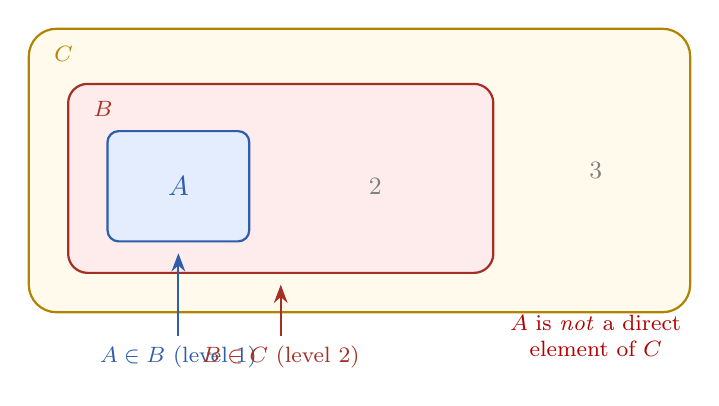
\begin{tikzpicture}[font=\small, >=Stealth]
  % Three nested boxes with clear level labels
  \fill[setC!8, rounded corners=10pt] (-0.2,-0.2) rectangle (8.2, 3.4);
  \draw[thick, setC!70!black, rounded corners=10pt] (-0.2,-0.2) rectangle (8.2, 3.4);
  \node[anchor=north west, font=\footnotesize\bfseries, setC!70!black] at (0, 3.3) {$C$};

  \fill[setB!10, rounded corners=7pt] (0.3, 0.3) rectangle (5.7, 2.7);
  \draw[thick, setB!70!black, rounded corners=7pt] (0.3, 0.3) rectangle (5.7, 2.7);
  \node[anchor=north west, font=\footnotesize\bfseries, setB!70!black] at (0.5, 2.6) {$B$};

  \fill[setA!15, rounded corners=4pt] (0.8, 0.7) rectangle (2.6, 2.1);
  \draw[thick, setA!70!black, rounded corners=4pt] (0.8, 0.7) rectangle (2.6, 2.1);
  \node[font=\bfseries, setA!70!black] at (1.7, 1.4) {$A$};

  % Other elements
  \node[font=\small, gray] at (4.2, 1.4) {$2$};
  \node[font=\small, gray] at (7.0, 1.6) {$3$};

  % Annotations
  \draw[<-, thick, setA!70!black] (1.7, 0.55) -- (1.7, -0.5)
    node[below, font=\footnotesize]{$A \in B$ (level 1)};
  \draw[<-, thick, setB!70!black] (3.0, 0.15) -- (3.0, -0.5)
    node[below, font=\footnotesize]{$B \in C$ (level 2)};
  \node[font=\footnotesize, red!70!black, align=center] at (7.0, -0.5)
    {$A$ is \emph{not} a direct\\element of $C$};
\end{tikzpicture}
\end{center}
\end{theorybox}

\begin{problembox}
Give examples of sets $A$, $B$, $C$ such that
$A \in B$, \;$B \in C$, \;but $A \notin C$.
\end{problembox}

\subsection*{Solution}
Let
\[
  A = 1, \qquad B = \{1, 2\}, \qquad C = \bigl\{\{1, 2\},\; 3\bigr\}.
\]

\begin{center}
\renewcommand{\arraystretch}{1.4}
\begin{tabular}{lll}
\toprule
\textbf{Condition} & \textbf{Check} & \textbf{Result} \\
\midrule
$A \in B$ & Is $1 \in \{1, 2\}$? & Yes $\checkmark$ \\
$B \in C$ & Is $\{1,2\} \in \bigl\{\{1,2\},\, 3\bigr\}$? & Yes $\checkmark$ \\
$A \notin C$ & Is $1 \in \bigl\{\{1,2\},\, 3\bigr\}$?
  The elements are $\{1,2\}$ and $3$. & $1 \notin C$ \;$\checkmark$ \\
\bottomrule
\end{tabular}
\end{center}

\textbf{Key insight.}\;
The number $1$ is an element of $B$, and $B$ is an element of $C$,
but the elements of $C$ are $\{1,2\}$ (a set) and $3$ (a number).
The number $1$ is neither of these, so $1 \notin C$.

% ══════════════════════════════════════════════════════════════════
\section{Problem 11 --- Mixing $\in$ and $\subseteq$}
% ══════════════════════════════════════════════════════════════════

\begin{theorybox}[Mixing $\in$ and $\subseteq$]
The two relations operate at different ``levels'':
\begin{itemize}[nosep]
  \item $A \subseteq B$: both sit at the same level---every element of $A$
        is also an element of $B$.
  \item $B \in C$: $B$ itself becomes an object inside $C$---a jump \emph{up} one level.
\end{itemize}

\begin{center}
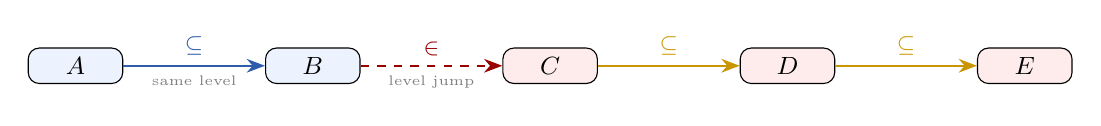
\begin{tikzpicture}[font=\small, >=Stealth, node distance=1.8cm]
  \node[draw, rounded corners, fill=setA!10, minimum width=1.2cm] (A) {$A$};
  \node[draw, rounded corners, fill=setA!10, minimum width=1.2cm, right=of A] (B) {$B$};
  \node[draw, rounded corners, fill=setB!10, minimum width=1.2cm, right=of B] (C) {$C$};
  \node[draw, rounded corners, fill=setB!10, minimum width=1.2cm, right=of C] (D) {$D$};
  \node[draw, rounded corners, fill=setB!10, minimum width=1.2cm, right=of D] (E) {$E$};

  \draw[->, thick, setA!70!black] (A) -- (B)
    node[midway, above, font=\footnotesize]{$\subseteq$}
    node[midway, below, font=\tiny, gray]{same level};
  \draw[->, thick, red!60!black, dashed] (B) -- (C)
    node[midway, above, font=\footnotesize]{$\in$}
    node[midway, below, font=\tiny, gray]{level jump};
  \draw[->, thick, setC!80!black] (C) -- (D)
    node[midway, above, font=\footnotesize]{$\subseteq$};
  \draw[->, thick, setC!80!black] (D) -- (E)
    node[midway, above, font=\footnotesize]{$\subseteq$};
\end{tikzpicture}
\end{center}
\end{theorybox}

\begin{problembox}
Give examples of sets $A, B, C, D, E$ satisfying:
\[
  A \subseteq B, \quad B \in C, \quad C \subseteq D, \quad D \subseteq E.
\]
\end{problembox}

\subsection*{Solution}

\[
  A = \{1\}, \quad B = \{1,2\}, \quad C = \bigl\{\{1,2\},\;3\bigr\}, \quad
  D = \bigl\{\{1,2\},\;3,\;4\bigr\}, \quad E = \bigl\{\{1,2\},\;3,\;4,\;5\bigr\}
\]

\begin{center}
\renewcommand{\arraystretch}{1.35}
\begin{tabular}{lcp{7.5cm}}
\toprule
\textbf{Condition} & \textbf{Type} & \textbf{Verification} \\
\midrule
$A \subseteq B$ & subset &
  Every element of $\{1\}$ is in $\{1,2\}$: $1 \in \{1,2\}$ \;\checkmark \\
$B \in C$ & membership &
  $\{1,2\}$ is listed as an element of $\bigl\{\{1,2\},3\bigr\}$ \;\checkmark \\
$C \subseteq D$ & subset &
  Elements $\{1,2\}$ and $3$ of $C$ are both in $D$ \;\checkmark \\
$D \subseteq E$ & subset &
  Elements $\{1,2\}$, $3$, $4$ of $D$ are all in $E$ \;\checkmark \\
\bottomrule
\end{tabular}
\end{center}

\textbf{Why this works.}\;
$\subseteq$ preserves the ``level'': $A$ and $B$ contain the same kind of objects (numbers).
The $\in$-step promotes $B$ to an object inside $C$, after which
$C$, $D$, $E$ all live at the higher level (their elements include sets like $\{1,2\}$).

% ══════════════════════════════════════════════════════════════════
\section{Problem 16 --- Describing Sets Under Operations}
% ══════════════════════════════════════════════════════════════════

\begin{theorybox}[Set Operations]
For subsets of a universal set $U$:

\smallskip
\begin{center}
\renewcommand{\arraystretch}{1.25}
\begin{tabular}{lcl}
\toprule
\textbf{Operation} & \textbf{Symbol} & \textbf{Definition} \\
\midrule
Complement & $\comp{A}$ & $\{x \in U \mid x \notin A\}$ \\
Set difference & $A \setminus B$ & $\{x \in A \mid x \notin B\}$ \\
Symmetric diff. & $A \symdiff B$ &
  $(A \setminus B) \cup (B \setminus A)$
  $=$ elements in exactly one of $A,\,B$ \\
\bottomrule
\end{tabular}
\end{center}

\begin{center}
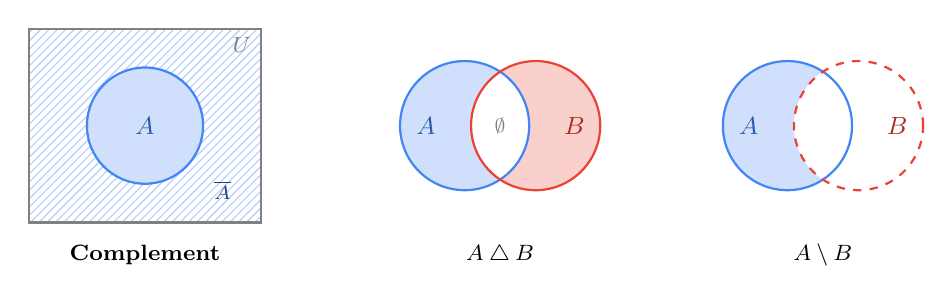
\begin{tikzpicture}[scale=0.82]
  % --- Complement ---
  \begin{scope}[xshift=0cm]
    % U background with hatching for complement
    \begin{scope}
      \clip (-1.8,-1.5) rectangle (1.8,1.5);
      \fill[pattern=north east lines, pattern color=setA!40]
           (-1.8,-1.5) rectangle (1.8,1.5);
      \fill[white] (0,0) circle (0.9);
    \end{scope}
    \fill[setA!25] (0,0) circle (0.9);
    \draw[thick, setA] (0,0) circle (0.9);
    \draw[thick, gray] (-1.8,-1.5) rectangle (1.8,1.5);
    \node[font=\footnotesize, gray] at (1.5,1.25) {$U$};
    \node[font=\small\bfseries, setA!70!black] at (0,0) {$A$};
    \node[font=\scriptsize, setA!50!black] at (1.2, -1.0) {$\comp{A}$};
    \node[font=\footnotesize\bfseries] at (0,-2.0) {Complement};
  \end{scope}

  % --- Symmetric Difference ---
  \begin{scope}[xshift=5.5cm]
    % A only (shade)
    \begin{scope}
      \clip (-0.55,0) circle (1);
      \fill[setA!25] (-2,-2) rectangle (2,2);
      \fill[white] (0.55,0) circle (1);
    \end{scope}
    % B only (shade)
    \begin{scope}
      \clip (0.55,0) circle (1);
      \fill[setB!25] (-2,-2) rectangle (2,2);
      \fill[white] (-0.55,0) circle (1);
    \end{scope}
    \draw[thick, setA] (-0.55,0) circle (1);
    \draw[thick, setB] (0.55,0) circle (1);
    \node[font=\small\bfseries, setA!70!black] at (-1.15,0) {$A$};
    \node[font=\small\bfseries, setB!70!black] at (1.15,0) {$B$};
    \node[font=\scriptsize] at (0, 0) {\color{gray}$\emptyset$};
    \node[font=\footnotesize\bfseries] at (0,-2.0) {$A \symdiff B$};
  \end{scope}

  % --- Set Difference ---
  \begin{scope}[xshift=10.5cm]
    % A minus B (shade A only)
    \begin{scope}
      \clip (-0.55,0) circle (1);
      \fill[setA!25] (-2,-2) rectangle (2,2);
      \fill[white] (0.55,0) circle (1);
    \end{scope}
    \draw[thick, setA] (-0.55,0) circle (1);
    \draw[thick, setB, dashed] (0.55,0) circle (1);
    \node[font=\small\bfseries, setA!70!black] at (-1.15,0) {$A$};
    \node[font=\small\bfseries, setB!70!black] at (1.15,0) {$B$};
    \node[font=\footnotesize\bfseries] at (0,-2.0) {$A \setminus B$};
  \end{scope}
\end{tikzpicture}
\end{center}
\end{theorybox}

\begin{problembox}
Let $\Z$ be the universal set. Define:
\begin{align*}
  A &= \{x \in \Z \mid \exists\, y \in \Z^+,\; x = 2y\}
      &&\text{(positive even integers: } 2, 4, 6, 8, \ldots) \\
  B &= \{x \in \Z \mid \exists\, y \in \Z^+,\; x = 2y - 1\}
      &&\text{(positive odd integers: } 1, 3, 5, 7, \ldots) \\
  C &= \{x \in \Z \mid x < 10\}
\end{align*}
Describe: \;$\comp{A}$,\; $A \symdiff B$,\; $\comp{C}$,\;
$A \setminus C$,\; $C \setminus (A \symdiff B)$.
\end{problembox}

\subsection*{Solution}

\paragraph{Visualising the sets on the number line.}

\begin{center}
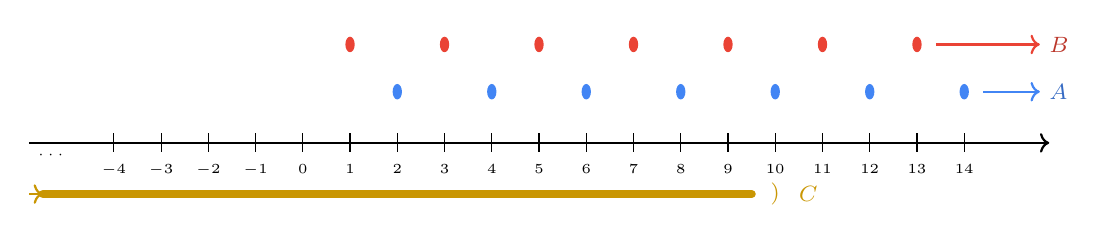
\begin{tikzpicture}[xscale=0.6, font=\small]
  % axis
  \draw[->, thick] (-5.8,0) -- (15.8,0);
  \foreach \x in {-4,-3,...,14} {
    \draw (\x, 0.12) -- (\x, -0.12);
    \node[below, font=\tiny] at (\x, -0.15) {$\x$};
  }
  \node[font=\tiny] at (-5.3, -0.15) {$\cdots$};

  % A: positive evens (blue dots)
  \foreach \x in {2,4,6,8,10,12,14}
    \fill[setA] (\x, 0.65) circle (2.8pt);
  \draw[->, setA, thick] (14.4, 0.65) -- (15.6, 0.65);
  \node[right, setA!80!black, font=\footnotesize] at (15.6, 0.65) {$A$};

  % B: positive odds (red dots)
  \foreach \x in {1,3,5,7,9,11,13}
    \fill[setB] (\x, 1.25) circle (2.8pt);
  \draw[->, setB, thick] (13.4, 1.25) -- (15.6, 1.25);
  \node[right, setB!80!black, font=\footnotesize] at (15.6, 1.25) {$B$};

  % C: x < 10 (yellow bar)
  \draw[setC!80!black, line width=3pt, line cap=round]
    (-5.5, -0.65) -- (9.5, -0.65);
  \draw[<-, setC!80!black, thick] (-5.5, -0.65) -- (-5.8, -0.65);
  \node[setC!80!black, font=\footnotesize] at (10.0, -0.65) {$)$};
  \node[right, setC!80!black, font=\footnotesize] at (10.3, -0.65) {$C$};
\end{tikzpicture}
\end{center}

\textbf{(a)\; $\comp{A}$:}\;
Everything in $\Z$ that is \emph{not} a positive even integer:
\[
  \boxed{\comp{A} = \{\ldots, -2, -1, 0\} \;\cup\; \{1, 3, 5, 7, \ldots\}
         = \bigl\{x \in \Z \mid x \le 0 \text{ or } x \text{ is odd}\bigr\}}
\]

\textbf{(b)\; $A \symdiff B$:}\;
Since $A \cap B = \emptyset$ (no integer is both positive-even and positive-odd):
\[
  A \symdiff B = A \cup B = \{1, 2, 3, 4, \ldots\}
  \qquad\Longrightarrow\qquad
  \boxed{A \symdiff B = \Z^+}
\]

\textbf{(c)\; $\comp{C}$:}\;
All integers $\ge 10$:
$\quad\boxed{\comp{C} = \{10, 11, 12, \ldots\}}$

\textbf{(d)\; $A \setminus C$:}\;
Positive evens that are $\ge 10$:
$\quad\boxed{A \setminus C = \{10, 12, 14, \ldots\} = \{2k \mid k \ge 5\}}$

\textbf{(e)\; $C \setminus (A \symdiff B)$:}\;
Remove all positive integers ($=A \symdiff B$) from $C$:
$\quad\boxed{C \setminus (A \symdiff B) = \{\ldots, -2, -1, 0\} = \{x \in \Z \mid x \le 0\}}$

% ══════════════════════════════════════════════════════════════════
\newpage
\section{Problem 20 --- Equivalent Characterizations of $\subseteq$}
% ══════════════════════════════════════════════════════════════════

\begin{theorybox}[Cyclic-Implication Proof Strategy]
To show three conditions $(a)$, $(b)$, $(c)$ are equivalent, it suffices to prove
a \textbf{cycle of implications}:
\[
  (a) \;\Longrightarrow\; (b) \;\Longrightarrow\; (c) \;\Longrightarrow\; (a).
\]
This is more efficient than proving all six pairwise implications directly.

\begin{center}
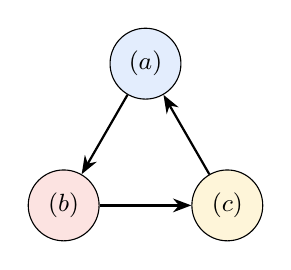
\begin{tikzpicture}[>=Stealth, font=\small]
  \node[draw, circle, minimum size=0.9cm, fill=setA!15] (a) at (90:1.2) {$(a)$};
  \node[draw, circle, minimum size=0.9cm, fill=setB!15] (b) at (210:1.2) {$(b)$};
  \node[draw, circle, minimum size=0.9cm, fill=setC!15] (c) at (330:1.2) {$(c)$};
  \draw[->, thick] (a) -- (b);
  \draw[->, thick] (b) -- (c);
  \draw[->, thick] (c) -- (a);
\end{tikzpicture}
\end{center}
\end{theorybox}

\begin{problembox}
Prove that for any subsets $A, B$ of universal set $U$,
the conditions in each group are equivalent:
\begin{enumerate}[nosep]
  \item $A \subseteq B \;\iff\; A \cup B = B \;\iff\; A \cap B = A$
  \item $A \cap B = \emptyset \;\iff\; A \subseteq \comp{B} \;\iff\; B \subseteq \comp{A}$
  \item $A \cup B = U \;\iff\; \comp{A} \subseteq B \;\iff\; \comp{B} \subseteq A$
\end{enumerate}
\end{problembox}

% ---- Part 1 ----
\subsection*{Part 1:\; $A \subseteq B \;\iff\; A \cup B = B \;\iff\; A \cap B = A$}

\begin{center}
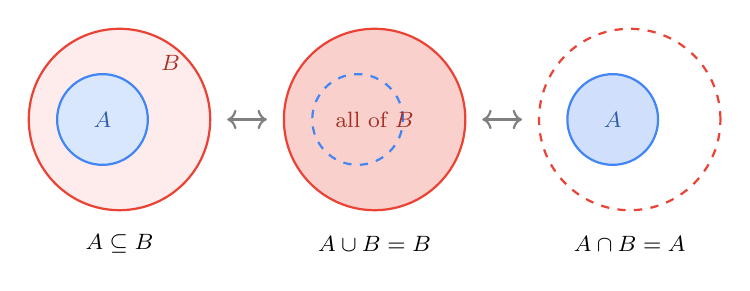
\begin{tikzpicture}[scale=0.72]
  % A subset B
  \draw[thick, setB, fill=setB!10] (0,0) circle (1.6);
  \draw[thick, setA, fill=setA!20] (-0.3,0) circle (0.8);
  \node[font=\footnotesize\bfseries, setA!70!black] at (-0.3,0) {$A$};
  \node[font=\footnotesize\bfseries, setB!70!black] at (0.9,1.0) {$B$};
  \node[font=\footnotesize] at (0, -2.2) {$A \subseteq B$};

  \begin{scope}[xshift=4.5cm]
    \draw[thick, setB, fill=setB!25] (0,0) circle (1.6);
    \draw[thick, setA, dashed] (-0.3,0) circle (0.8);
    \node[font=\footnotesize] at (0, -2.2) {$A \cup B = B$};
    \node[font=\footnotesize, setB!70!black] at (0,0) {all of $B$};
  \end{scope}

  \begin{scope}[xshift=9cm]
    \draw[thick, setB, dashed] (0,0) circle (1.6);
    \draw[thick, setA, fill=setA!25] (-0.3,0) circle (0.8);
    \node[font=\footnotesize] at (0, -2.2) {$A \cap B = A$};
    \node[font=\footnotesize, setA!70!black] at (-0.3,0) {$A$};
  \end{scope}

  % arrows between diagrams
  \draw[<->, thick, gray] (1.9, 0) -- (2.6, 0);
  \draw[<->, thick, gray] (6.4, 0) -- (7.1, 0);
\end{tikzpicture}
\end{center}

\textbf{$(a) \Rightarrow (b)$:}\;
$A \subseteq B \;\Longrightarrow\; A \cup B = B$.

($\supseteq$)\; $B \subseteq A \cup B$ always.

($\subseteq$)\; Let $x \in A \cup B$.
Then $x \in A$ or $x \in B$.
If $x \in A$, then $A \subseteq B$ gives $x \in B$.
Either way, $x \in B$. \qed

\textbf{$(b) \Rightarrow (c)$:}\;
$A \cup B = B \;\Longrightarrow\; A \cap B = A$.

($\subseteq$)\; $A \cap B \subseteq A$ always.

($\supseteq$)\; Let $x \in A$.
Then $x \in A \cup B = B$, so $x \in B$.
Hence $x \in A \cap B$. \qed

\textbf{$(c) \Rightarrow (a)$:}\;
$A \cap B = A \;\Longrightarrow\; A \subseteq B$.

Let $x \in A$. Then $x \in A = A \cap B$, so $x \in B$. \qed

% ---- Part 2 ----
\subsection*{Part 2:\; $A \cap B = \emptyset \;\iff\; A \subseteq \comp{B} \;\iff\; B \subseteq \comp{A}$}

\begin{center}
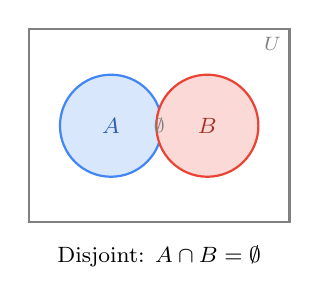
\begin{tikzpicture}[scale=0.72]
  \draw[thick, gray] (-2.3,-1.7) rectangle (2.3,1.7);
  \node[gray, font=\scriptsize] at (2.0,1.45) {$U$};
  \draw[thick, setA, fill=setA!20] (-0.85,0) circle (0.9);
  \draw[thick, setB, fill=setB!20] (0.85,0) circle (0.9);
  \node[font=\footnotesize\bfseries, setA!70!black] at (-0.85,0) {$A$};
  \node[font=\footnotesize\bfseries, setB!70!black] at (0.85,0) {$B$};
  \node[font=\footnotesize] at (0,-2.3) {Disjoint: $A \cap B = \emptyset$};
  \node[font=\scriptsize, gray] at (0, 0) {$\emptyset$};
\end{tikzpicture}
\end{center}

\textbf{$(a) \Rightarrow (b)$:}\;
$A \cap B = \emptyset \;\Longrightarrow\; A \subseteq \comp{B}$.

Let $x \in A$. If $x \in B$, then $x \in A \cap B = \emptyset$---contradiction.
So $x \notin B$, i.e.\ $x \in \comp{B}$. \qed

\textbf{$(b) \Rightarrow (c)$:}\;
$A \subseteq \comp{B} \;\Longrightarrow\; B \subseteq \comp{A}$.

Let $x \in B$. If $x \in A$, then $x \in \comp{B}$ (since $A \subseteq \comp{B}$),
so $x \notin B$---contradiction. Hence $x \notin A$, i.e.\ $x \in \comp{A}$. \qed

\textbf{$(c) \Rightarrow (a)$:}\;
$B \subseteq \comp{A} \;\Longrightarrow\; A \cap B = \emptyset$.

Suppose $x \in A \cap B$. Then $x \in B \subseteq \comp{A}$,
so $x \notin A$---contradicting $x \in A \cap B$. \qed

% ---- Part 3 ----
\subsection*{Part 3:\; $A \cup B = U \;\iff\; \comp{A} \subseteq B \;\iff\; \comp{B} \subseteq A$}

\begin{center}
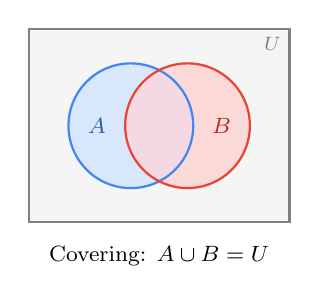
\begin{tikzpicture}[scale=0.72]
  % Shading: entire U is covered
  \draw[thick, gray, fill=gray!8] (-2.3,-1.7) rectangle (2.3,1.7);
  \node[gray, font=\scriptsize] at (2.0,1.45) {$U$};
  \fill[setA!20] (-0.5,0) circle (1.1);
  \fill[setB!20] (0.5,0) circle (1.1);
  % overlap
  \begin{scope}
    \clip (-0.5,0) circle (1.1);
    \fill[purple!15] (0.5,0) circle (1.1);
  \end{scope}
  \draw[thick, setA] (-0.5,0) circle (1.1);
  \draw[thick, setB] (0.5,0) circle (1.1);
  \node[font=\footnotesize\bfseries, setA!70!black] at (-1.1,0) {$A$};
  \node[font=\footnotesize\bfseries, setB!70!black] at (1.1,0) {$B$};
  \node[font=\footnotesize] at (0,-2.3) {Covering: $A \cup B = U$};
\end{tikzpicture}
\end{center}

\textbf{$(a) \Rightarrow (b)$:}\;
$A \cup B = U \;\Longrightarrow\; \comp{A} \subseteq B$.

Let $x \in \comp{A}$, so $x \notin A$.
Since $x \in U = A \cup B$ and $x \notin A$, we must have $x \in B$. \qed

\textbf{$(b) \Rightarrow (c)$:}\;
$\comp{A} \subseteq B \;\Longrightarrow\; \comp{B} \subseteq A$.

Let $x \in \comp{B}$, so $x \notin B$.
If $x \notin A$, then $x \in \comp{A} \subseteq B$, giving $x \in B$---contradiction.
So $x \in A$. \qed

\textbf{$(c) \Rightarrow (a)$:}\;
$\comp{B} \subseteq A \;\Longrightarrow\; A \cup B = U$.

Let $x \in U$. Either $x \in B$ (then $x \in A \cup B$)
or $x \notin B$ (then $x \in \comp{B} \subseteq A$, so $x \in A \cup B$).
Since also $A \cup B \subseteq U$, we get $A \cup B = U$. \qed

% ══════════════════════════════════════════════════════════════════
\newpage
\section{Problem 54.3 --- $(A \cup B) \setminus C = (A \setminus C) \cup (B \setminus C)$}
% ══════════════════════════════════════════════════════════════════

\begin{theorybox}[Set Difference Distributes Over Union]
Mental model: ``$X \setminus C$'' means
``start with $X$, \textbf{remove} everything in $C$.''

Removing $C$ from a union is the same as removing $C$ from each piece separately,
then taking the union of the remainders.

\begin{center}
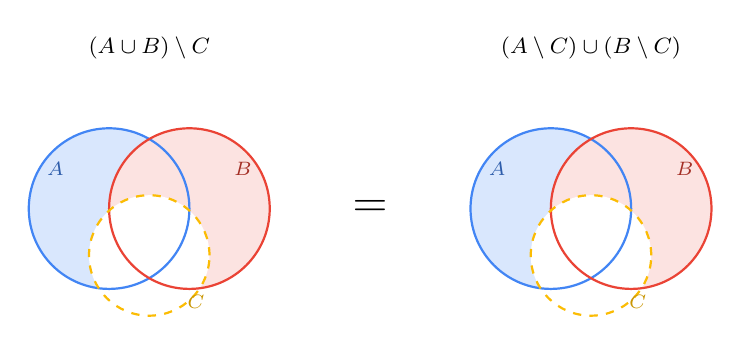
\begin{tikzpicture}[scale=0.85]
  % --- LHS ---
  \begin{scope}[xshift=0cm]
    \node[font=\footnotesize\bfseries] at (0, 2.4) {$(A \cup B) \setminus C$};
    % shade A\C
    \begin{scope}
      \clip (-0.6,0) circle (1.2);
      \fill[setA!20] (-3,-3) rectangle (3,3);
    \end{scope}
    % shade B\C
    \begin{scope}
      \clip (0.6,0) circle (1.2);
      \fill[setB!15] (-3,-3) rectangle (3,3);
    \end{scope}
    % cut out C
    \fill[white] (0, -0.7) circle (0.9);

    \draw[thick, setA] (-0.6, 0) circle (1.2);
    \draw[thick, setB] (0.6, 0) circle (1.2);
    \draw[thick, setC, dashed] (0, -0.7) circle (0.9);
    \node[font=\scriptsize, setA!70!black] at (-1.4, 0.6) {$A$};
    \node[font=\scriptsize, setB!70!black] at (1.4, 0.6) {$B$};
    \node[font=\scriptsize, setC!80!black] at (0.7, -1.4) {$C$};
  \end{scope}

  \node[font=\LARGE] at (3.3, 0) {$=$};

  % --- RHS ---
  \begin{scope}[xshift=6.6cm]
    \node[font=\footnotesize\bfseries] at (0, 2.4) {$(A \setminus C) \cup (B \setminus C)$};
    % shade A\C
    \begin{scope}
      \clip (-0.6,0) circle (1.2);
      \fill[setA!20] (-3,-3) rectangle (3,3);
    \end{scope}
    % shade B\C
    \begin{scope}
      \clip (0.6,0) circle (1.2);
      \fill[setB!15] (-3,-3) rectangle (3,3);
    \end{scope}
    % cut out C
    \fill[white] (0, -0.7) circle (0.9);

    \draw[thick, setA] (-0.6, 0) circle (1.2);
    \draw[thick, setB] (0.6, 0) circle (1.2);
    \draw[thick, setC, dashed] (0, -0.7) circle (0.9);
    \node[font=\scriptsize, setA!70!black] at (-1.4, 0.6) {$A$};
    \node[font=\scriptsize, setB!70!black] at (1.4, 0.6) {$B$};
    \node[font=\scriptsize, setC!80!black] at (0.7, -1.4) {$C$};
  \end{scope}
\end{tikzpicture}
\end{center}
Both diagrams shade exactly the same region---the parts of $A$ and $B$
that fall outside $C$.
\end{theorybox}

\begin{problembox}
Prove:\quad $(A \cup B) \setminus C = (A \setminus C) \cup (B \setminus C)$.
\end{problembox}

\subsection*{Solution}

Let $x$ be arbitrary:
\begin{align*}
  x \in (A \cup B) \setminus C
  &\iff x \in (A \cup B) \;\land\; x \notin C \\
  &\iff (x \in A \;\lor\; x \in B) \;\land\; x \notin C \\
  &\iff (x \in A \land x \notin C)
        \;\lor\; (x \in B \land x \notin C)
        && \text{($\land$ distributes over $\lor$)} \\
  &\iff x \in (A \setminus C) \;\lor\; x \in (B \setminus C) \\
  &\iff x \in (A \setminus C) \cup (B \setminus C).
\end{align*}
Every step is $\iff$, so the sets are equal. \qed

\textbf{Logic correspondence.}\;
The key step uses the propositional law
$p \land (q \lor r) \iff (p \land q) \lor (p \land r)$,
where $p = (x \notin C)$,\; $q = (x \in A)$,\; $r = (x \in B)$.

% ══════════════════════════════════════════════════════════════════
\newpage
\section{Problem 54.11 --- $\cap$ Distributes Over $\triangle$}
% ══════════════════════════════════════════════════════════════════

\begin{theorybox}[Intersection Distributes Over Symmetric Difference]
Recall:\; $X \symdiff Y = \{x \mid x \text{ belongs to exactly one of } X, Y\}$.

\medskip
The identity $A \cap (B \symdiff C) = (A \cap B) \symdiff (A \cap C)$
says:
\begin{quote}
\textit{``The part of $A$ that sees exactly one of $B, C$''}
equals
\textit{``exactly one of ($A$'s overlap with $B$) and ($A$'s overlap with $C$).''}
\end{quote}

\begin{center}
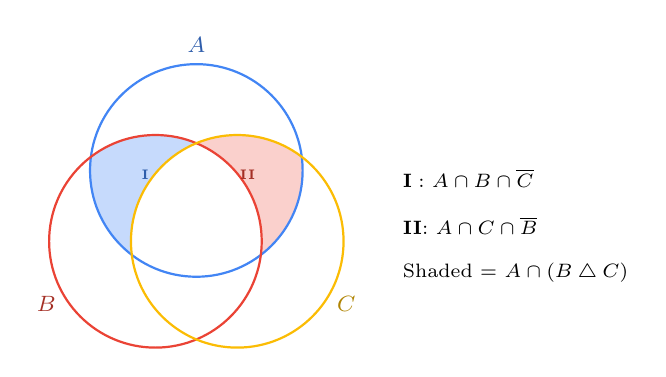
\begin{tikzpicture}[scale=1.0]
  % Three-set Venn with regions shaded for A ∩ (B △ C)
  \def\rr{1.35}
  \def\sep{0.6}
  \coordinate (cA) at (90:\sep);
  \coordinate (cB) at (210:\sep);
  \coordinate (cC) at (330:\sep);

  % Region: A ∩ B only (not C) --- shade
  \begin{scope}
    \clip (cA) circle (\rr);
    \clip (cB) circle (\rr);
    \fill[setA!30] (-3,-3) rectangle (3,3);
    \fill[white] (cC) circle (\rr);
  \end{scope}

  % Region: A ∩ C only (not B) --- shade
  \begin{scope}
    \clip (cA) circle (\rr);
    \clip (cC) circle (\rr);
    \fill[setB!25] (-3,-3) rectangle (3,3);
    \fill[white] (cB) circle (\rr);
  \end{scope}

  % Outlines
  \draw[thick, setA] (cA) circle (\rr);
  \draw[thick, setB] (cB) circle (\rr);
  \draw[thick, setC] (cC) circle (\rr);

  \node[font=\footnotesize\bfseries, setA!70!black] at (90:2.2) {$A$};
  \node[font=\footnotesize\bfseries, setB!70!black] at (210:2.2) {$B$};
  \node[font=\footnotesize\bfseries, setC!70!black] at (330:2.2) {$C$};

  % Labels for shaded regions
  \node[font=\tiny, setA!70!black] at (-0.65, 0.55) {\textbf{I}};
  \node[font=\tiny, setB!70!black] at (0.65, 0.55) {\textbf{II}};

  % Legend
  \node[font=\scriptsize, anchor=west] at (2.5, 0.5)
    {\textbf{I}\;: $A \cap B \cap \comp{C}$};
  \node[font=\scriptsize, anchor=west] at (2.5, -0.1)
    {\textbf{II}: $A \cap C \cap \comp{B}$};
  \node[font=\scriptsize, anchor=west] at (2.5, -0.7)
    {Shaded $=$ $A \cap (B \symdiff C)$};
\end{tikzpicture}
\end{center}

\medskip
\textbf{Algebraic analogy.}\;
Under the correspondence $\cap \leftrightarrow \cdot$ and
$\symdiff \leftrightarrow +\!\pmod{2}$,
the power set $(\mathcal{P}(U),\,\symdiff,\,\cap)$ forms a
commutative ring. This identity is the ring distributive law.
\end{theorybox}

\begin{problembox}
Prove:\quad $A \cap (B \symdiff C) = (A \cap B) \symdiff (A \cap C)$.
\end{problembox}

\subsection*{Solution}

Let $x$ be arbitrary. We expand both sides to the same logical form.

\textbf{Left-hand side:}
\begin{align*}
  x \in A \cap (B \symdiff C)
  &\iff x \in A \;\land\; x \in B \symdiff C \\
  &\iff x \in A \;\land\;
        \bigl[(x \in B \land x \notin C)
        \;\lor\; (x \notin B \land x \in C)\bigr] \\
  &\iff \underbrace{(x \in A \land x \in B \land x \notin C)}_{\text{case 1}}
        \;\lor\;
        \underbrace{(x \in A \land x \notin B \land x \in C)}_{\text{case 2}}
        \tag{$\star$}
\end{align*}

\textbf{Right-hand side:}
\begin{align*}
  x \in (A \cap B) \symdiff (A \cap C)
  &\iff \bigl[x \in A \cap B \;\land\; x \notin A \cap C\bigr]
        \;\lor\;
        \bigl[x \notin A \cap B \;\land\; x \in A \cap C\bigr]
\end{align*}

\emph{First disjunct:}\; $x \in A \cap B$ and $x \notin A \cap C$.
\begin{itemize}[nosep]
  \item $x \in A \cap B \;\Longrightarrow\; x \in A$ and $x \in B$.
  \item $x \notin A \cap C$ means $\lnot(x \in A \land x \in C)$.
        Since $x \in A$, this forces $x \notin C$.
  \item Combined: $x \in A,\; x \in B,\; x \notin C$ \;(= case 1).
\end{itemize}

\emph{Second disjunct:}\; $x \notin A \cap B$ and $x \in A \cap C$.
\begin{itemize}[nosep]
  \item $x \in A \cap C \;\Longrightarrow\; x \in A$ and $x \in C$.
  \item $x \notin A \cap B$ means $\lnot(x \in A \land x \in B)$.
        Since $x \in A$, this forces $x \notin B$.
  \item Combined: $x \in A,\; x \notin B,\; x \in C$ \;(= case 2).
\end{itemize}

Both sides reduce to ($\star$), so:
\[
  A \cap (B \symdiff C) = (A \cap B) \symdiff (A \cap C).
  \qquad\blacksquare
\]

% ══════════════════════════════════════════════════════════════════
\newpage
\section{Problem 58 --- $A \times B = B \times A \;\Longrightarrow\; A = B$}
% ══════════════════════════════════════════════════════════════════

\begin{theorybox}[Cartesian Product]
\[
  A \times B = \{(a,b) \mid a \in A,\; b \in B\}.
\]
Order in the pair matters: $(a, b) \neq (b, a)$ when $a \neq b$.

\begin{center}
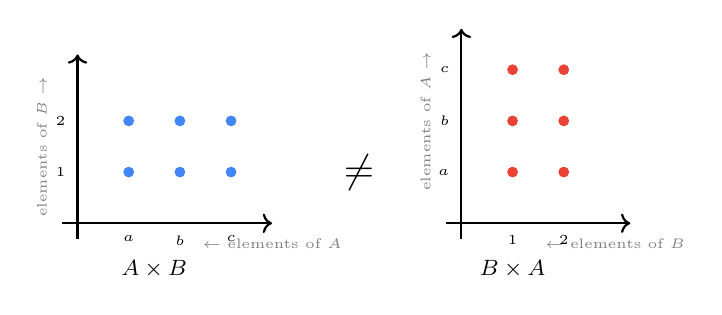
\begin{tikzpicture}[scale=0.65, font=\small]
  % A x B
  \begin{scope}
    \draw[->, thick] (-0.3,0) -- (3.8,0);
    \draw[->, thick] (0,-0.3) -- (0,3.3);
    % grid dots
    \foreach \x/\lx in {1/$a$, 2/$b$, 3/$c$} {
      \node[below, font=\tiny] at (\x, -0.05) {\lx};
      \foreach \y in {1,2} {
        \fill[setA] (\x, \y) circle (3pt);
      }
    }
    \foreach \y/\ly in {1/$1$, 2/$2$} {
      \node[left, font=\tiny] at (-0.05, \y) {\ly};
    }
    \node[font=\footnotesize\bfseries] at (1.5, -0.9) {$A \times B$};
    \node[font=\tiny, gray] at (3.8, -0.4) {$\leftarrow$ elements of $A$};
    \node[font=\tiny, gray, rotate=90] at (-0.7, 1.5) {elements of $B$ $\rightarrow$};
  \end{scope}

  \node[font=\Large] at (5.5, 1) {$\neq$};

  % B x A
  \begin{scope}[xshift=7.5cm]
    \draw[->, thick] (-0.3,0) -- (3.3,0);
    \draw[->, thick] (0,-0.3) -- (0,3.8);
    \foreach \x/\lx in {1/$1$, 2/$2$} {
      \node[below, font=\tiny] at (\x, -0.05) {\lx};
      \foreach \y in {1,2,3} {
        \fill[setB] (\x, \y) circle (3pt);
      }
    }
    \foreach \y/\ly in {1/$a$, 2/$b$, 3/$c$} {
      \node[left, font=\tiny] at (-0.05, \y) {\ly};
    }
    \node[font=\footnotesize\bfseries] at (1, -0.9) {$B \times A$};
    \node[font=\tiny, gray] at (3.0, -0.4) {$\leftarrow$ elements of $B$};
    \node[font=\tiny, gray, rotate=90] at (-0.7, 2) {elements of $A$ $\rightarrow$};
  \end{scope}
\end{tikzpicture}
\end{center}

When $A \neq B$, the grids have different shapes, so $A \times B \neq B \times A$.
\end{theorybox}

\begin{problembox}
Prove that $A \times B = B \times A$ implies $A = B$.

\smallskip
\textit{Note:} More precisely, $A \times B = B \times A$ implies
$A = B$, or $A = \emptyset$, or $B = \emptyset$.
\end{problembox}

\subsection*{Solution}

Assume $A \times B = B \times A$ with $A \neq \emptyset$ and $B \neq \emptyset$.
We show $A \subseteq B$ and $B \subseteq A$.

\textbf{$A \subseteq B$:}\;
Let $a \in A$. Since $B \neq \emptyset$, pick some $b \in B$.
\[
  (a, b) \in A \times B = B \times A
  \quad\Longrightarrow\quad
  \text{first component } a \in B.
\]
Since $a$ was arbitrary, $A \subseteq B$.

\textbf{$B \subseteq A$:}\;
Let $b \in B$. Since $A \neq \emptyset$, pick some $a \in A$.
\[
  (b, a) \in B \times A = A \times B
  \quad\Longrightarrow\quad
  \text{first component } b \in A.
\]
Since $b$ was arbitrary, $B \subseteq A$.

By antisymmetry of $\subseteq$:
$A \subseteq B \;\land\; B \subseteq A \;\Longrightarrow\; A = B$.
\qed

\textbf{Why non-emptiness matters.}\;
If $A = \emptyset$ and $B = \{1\}$, then
$A \times B = \emptyset = B \times A$,
but $A \neq B$.
We cannot ``pick $b \in B$'' if $B = \emptyset$, so the argument breaks down.

% ══════════════════════════════════════════════════════════════════
\newpage
\section{Problem 60 --- $\times$ Distributes Over Set Operations}
% ══════════════════════════════════════════════════════════════════

\begin{theorybox}[$\times$ Distributes Over $\cup$, $\cap$, $\setminus$]
All three proofs follow the same three-step recipe:
\begin{enumerate}[nosep, label=(\arabic*)]
  \item \textbf{Unpack:}\; $(x,y) \in A \times B \iff x \in A \land y \in B$.
  \item \textbf{Apply a propositional-logic law} ($\land/\lor$ distribution,
        or negation).
  \item \textbf{Repack} into set notation.
\end{enumerate}

The operation in the second component ``passes through'' $\times$:
\[
  A \times (B \;\diamond\; C) = (A \times B) \;\diamond\; (A \times C)
  \qquad \text{for } \diamond \in \{\cup,\,\cap,\,\setminus\}.
\]
Mirror identities $(B \;\diamond\; C) \times A$ work the same way on the
\emph{first} component.
We prove the three non-mirror versions; the mirrors follow by swapping $x \leftrightarrow y$.

\begin{center}
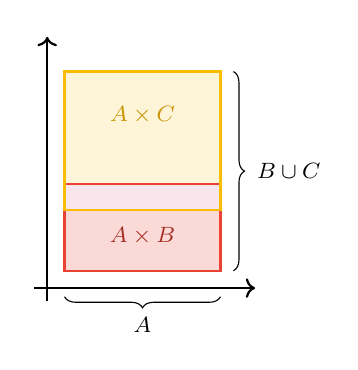
\begin{tikzpicture}[scale=0.55, font=\small]
  % A × (B ∪ C) as rectangular regions
  \draw[->, thick] (-0.3,0) -- (4.8,0) node[below, font=\footnotesize]{};
  \draw[->, thick] (0,-0.3) -- (0,5.8) node[left, font=\footnotesize]{};

  \fill[setB!20] (0.4, 0.4) rectangle (4.0, 2.4);
  \fill[setC!15] (0.4, 1.8) rectangle (4.0, 5.0);
  \fill[purple!10] (0.4, 1.8) rectangle (4.0, 2.4); % overlap

  \draw[thick, setB] (0.4, 0.4) rectangle (4.0, 2.4);
  \draw[thick, setC] (0.4, 1.8) rectangle (4.0, 5.0);

  \node[font=\footnotesize, setB!70!black] at (2.2, 1.2) {$A \times B$};
  \node[font=\footnotesize, setC!80!black] at (2.2, 4.0) {$A \times C$};

  \draw[decorate, decoration={brace, amplitude=4pt, mirror}]
    (4.3, 0.4) -- (4.3, 5.0)
    node[midway, right=5pt, font=\footnotesize]{$B \cup C$};
  \draw[decorate, decoration={brace, amplitude=4pt, mirror}]
    (0.4, -0.2) -- (4.0, -0.2)
    node[midway, below=4pt, font=\footnotesize]{$A$};
\end{tikzpicture}
\end{center}
\end{theorybox}

\begin{problembox}
Prove the following identities:
\begin{enumerate}[nosep]
  \item $A \times (B \cup C) = (A \times B) \cup (A \times C)$
  \item[3.] $A \times (B \cap C) = (A \times B) \cap (A \times C)$
  \item[5.] $A \times (B \setminus C) = (A \times B) \setminus (A \times C)$
\end{enumerate}
\end{problembox}

% ---- Identity 1 ----
\subsection*{Identity 1:\; $A \times (B \cup C) = (A \times B) \cup (A \times C)$}

Let $(x, y)$ be an arbitrary ordered pair:
\begin{align*}
  (x,y) \in A \times (B \cup C)
  &\iff x \in A \;\land\; y \in B \cup C \\
  &\iff x \in A \;\land\; (y \in B \;\lor\; y \in C) \\
  &\iff (x \in A \land y \in B)
        \;\lor\; (x \in A \land y \in C)
        && \text{($\land$ dist.\ over $\lor$)} \\
  &\iff (x,y) \in A \times B \;\lor\; (x,y) \in A \times C \\
  &\iff (x,y) \in (A \times B) \cup (A \times C).
  \qquad \blacksquare
\end{align*}

% ---- Identity 3 ----
\subsection*{Identity 3:\; $A \times (B \cap C) = (A \times B) \cap (A \times C)$}

Let $(x, y)$ be an arbitrary ordered pair:
\begin{align*}
  (x,y) \in A \times (B \cap C)
  &\iff x \in A \;\land\; y \in B \cap C \\
  &\iff x \in A \;\land\; y \in B \;\land\; y \in C \\
  &\iff (x \in A \land y \in B)
        \;\land\; (x \in A \land y \in C)
        && \text{(idempotency of $\land$)} \\
  &\iff (x,y) \in A \times B \;\land\; (x,y) \in A \times C \\
  &\iff (x,y) \in (A \times B) \cap (A \times C).
  \qquad \blacksquare
\end{align*}

% ---- Identity 5 ----
\subsection*{Identity 5:\; $A \times (B \setminus C) = (A \times B) \setminus (A \times C)$}

Let $(x, y)$ be an arbitrary ordered pair:
\begin{align*}
  (x,y) \in A \times (B \setminus C)
  &\iff x \in A \;\land\; y \in B \;\land\; y \notin C \\[4pt]
  &\iff \underbrace{(x \in A \land y \in B)}_{\displaystyle (x,y)\in A\times B}
        \;\;\land\;\;
        \underbrace{\lnot(x \in A \land y \in C)}_{\displaystyle (x,y)\notin A\times C}
        \tag{$\star$} \\[4pt]
  &\iff (x,y) \in (A \times B) \setminus (A \times C).
\end{align*}

\textit{Justification of $(\star)$:}\;
We need
$(p \land q \land \lnot r)
 \iff
(p \land q) \land \lnot(p \land r)$,
where $p = (x \in A)$, $q = (y \in B)$, $r = (y \in C)$.

$(\Rightarrow)$\;
$p, q, \lnot r$ all hold, so $p \land q$ holds.
Since $\lnot r$, the conjunction $p \land r$ is false,
so $\lnot(p \land r)$ holds.

$(\Leftarrow)$\;
From $p \land q$ we have $p$ and $q$.
From $\lnot(p \land r)$ and $p$, we get $\lnot r$.
\qed

\bigskip
\begin{answerbox}
\centering
Identities 2, 4, 6 are the mirror versions
$(B \;\diamond\; C) \times A = (B \times A) \;\diamond\; (C \times A)$
for $\diamond \in \{\cup, \cap, \setminus\}$.
Replace ``$x \in A$'' with ``$y \in A$'' throughout---the proofs are identical.
\end{answerbox}

\end{document}
